В качестве апробации разработанных алгоритмов моделирования (см. \ref{sec:source_section}, \ref{sec:slits_section})
были проведены расчеты для экспериментальной схемы изображенной на рис. \ref{ris:for_slits_scan_a}.

\begin{figure}[H]
  \centering
  \subfloat[]{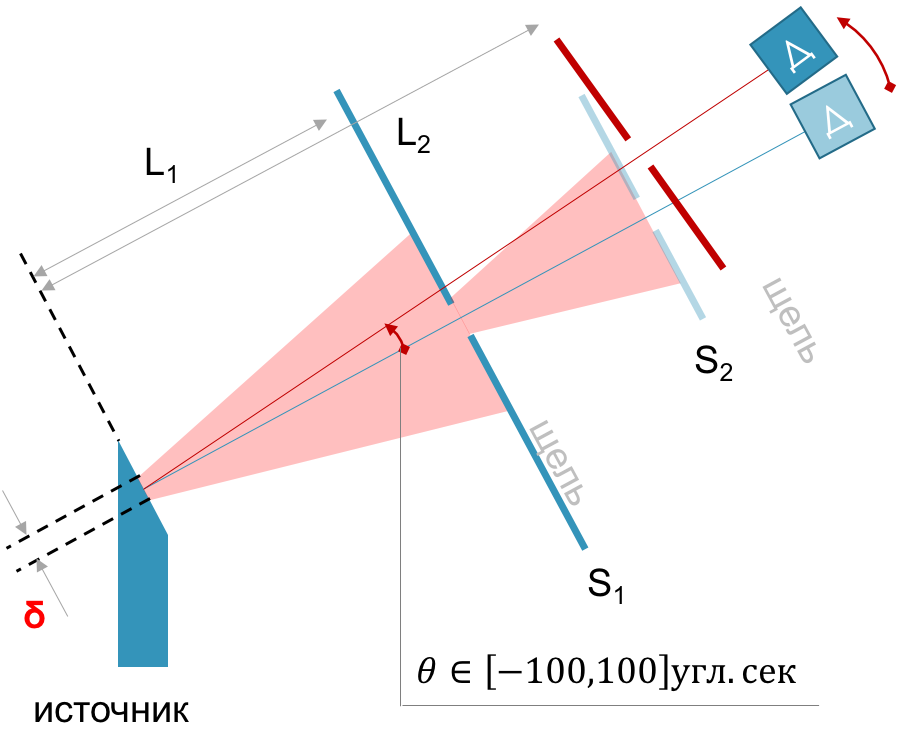
\includegraphics[width=0.52\textwidth]{images/for_slits_scan.png} \label{ris:for_slits_scan_a}}
  \hfill
  \subfloat[]{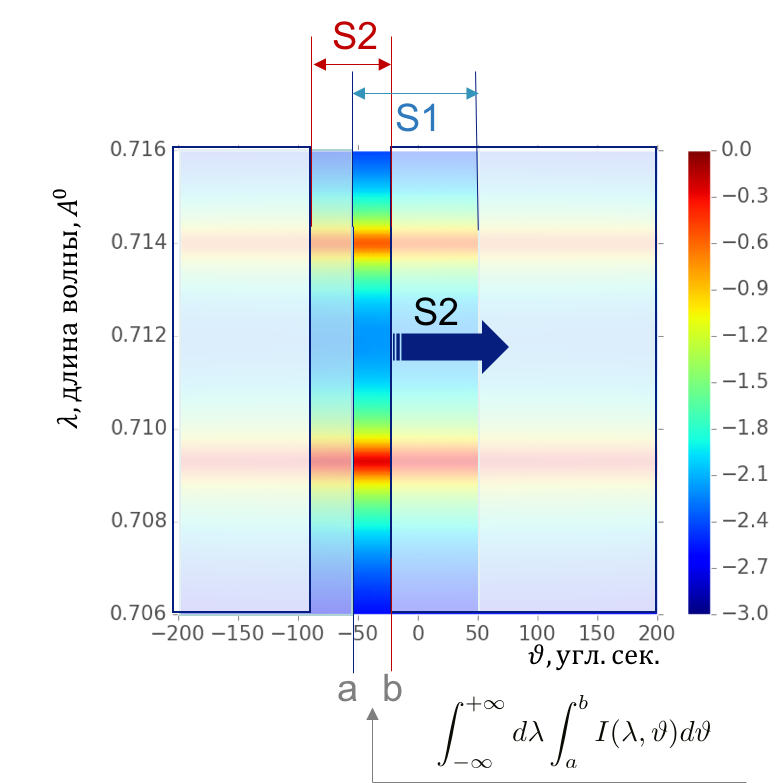
\includegraphics[width=0.45\textwidth]{images/for_slits_scan_int.png}}
  \caption{ (a) Схема эксперимента в остутствии отражающих элементов, (b) принцип интегрирования в
  случае точечного источника рентгеновского излучения, для случая протяженного см. (\ref{sec:calc_slits_ability})}
  \label{ris:for_slits_scan}

\end{figure}
В виду отсутствия линейного детектора для прямого наблюдения углового распределения интенсивности рентгеновского
пучка после его прохождения через систему щелевых устройств (рис. \ref{ris:for_slits_scan_a}),
возникает необходимость изменять угловое положение второго щелевого устройства (S2) и измерять суммарную интенсивность
за ним.

\begin{figure}[H]
  \centering
  \subfloat[]{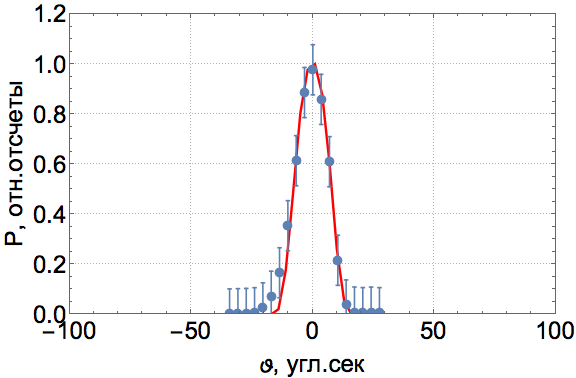
\includegraphics[width=0.3\textwidth]{images/zero_exp_20_40.png}}%$S_1 = 20$ мкм; $S_2 = 40$ мкм;
  \hfill
  \subfloat[]{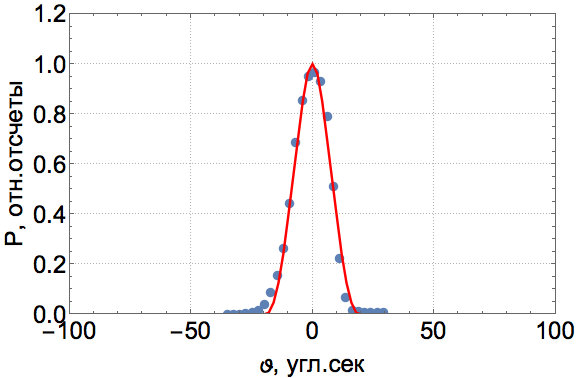
\includegraphics[width=0.3\textwidth]{images/zero_exp_40_40.png}}%$S_1 = 40$ мкм; $S_2 = 40$ мкм;
  \hfill
  \subfloat[]{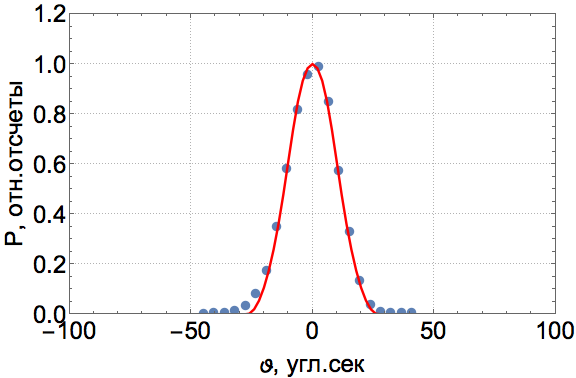
\includegraphics[width=0.3\textwidth]{images/zero_exp_50_100.png}} %$S_1 = 50$ мкм; $S_2 = 100$ мкм;
  \hfill
  % \subfloat[$S_1 = 60$ мкм; $S_2 = 40$ мкм;]{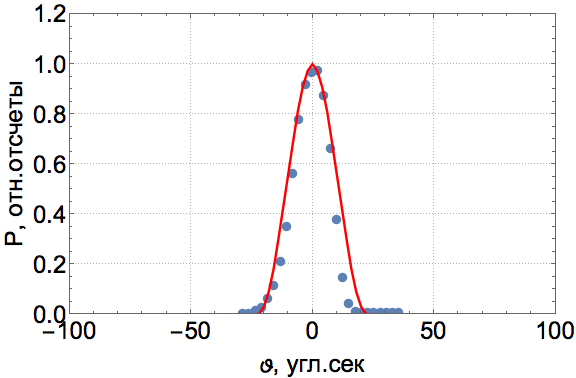
\includegraphics[width=0.3\textwidth]{images/zero_exp_60_40.png}}
  % \hfill
  \subfloat[]{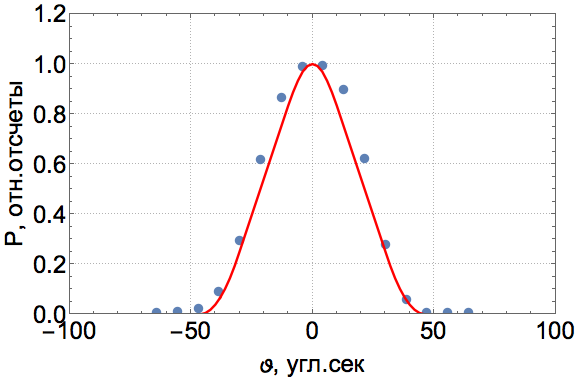
\includegraphics[width=0.3\textwidth]{images/zero_exp_100_200.png}} %$S_1 = 100$ мкм; $S_2 = 200$ мкм;
  \hfill
  \subfloat[]{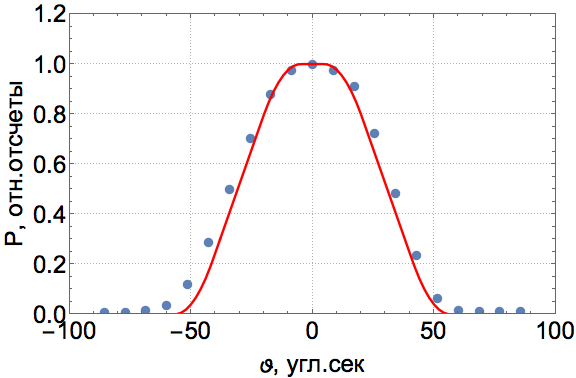
\includegraphics[width=0.3\textwidth]{images/zero_exp_100_300.png}} %$S_1 = 100$ мкм; $S_2 = 300$ мкм;
  \hfill
  \subfloat[]{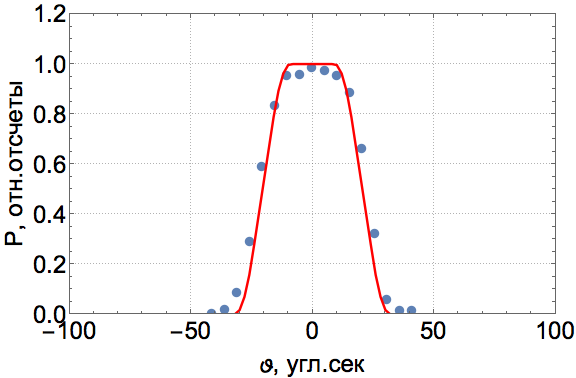
\includegraphics[width=0.3\textwidth]{images/zero_exp_200_20.png}} %$S_1 = 200$ мкм; $S_2 = 20$ мкм;
  \hfill
  \subfloat[]{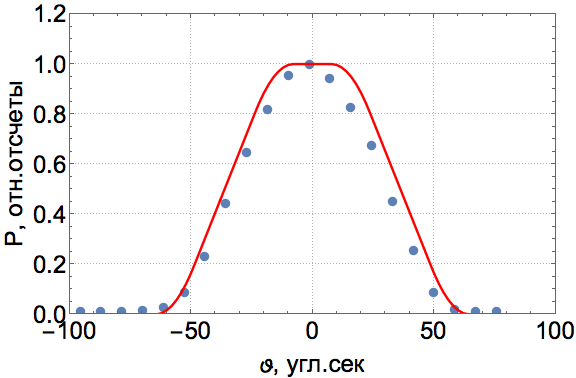
\includegraphics[width=0.3\textwidth]{images/zero_exp_200_200.png}} %$S_1 = 200$ мкм; $S_2 = 200$ мкм;
  \hfill
  \subfloat[]{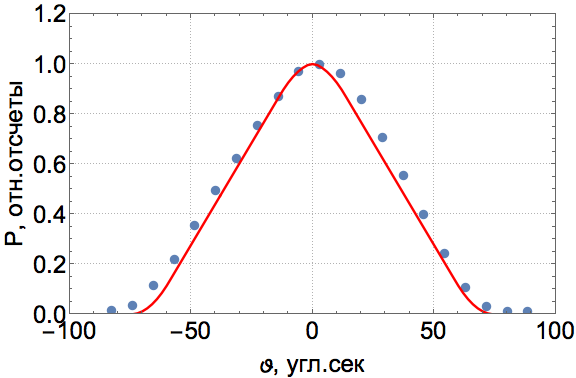
\includegraphics[width=0.3\textwidth]{images/zero_exp_200_300.png}} %$S_1 = 200$ мкм; $S_2 = 300$ мкм;
  \hfill
  \subfloat[]{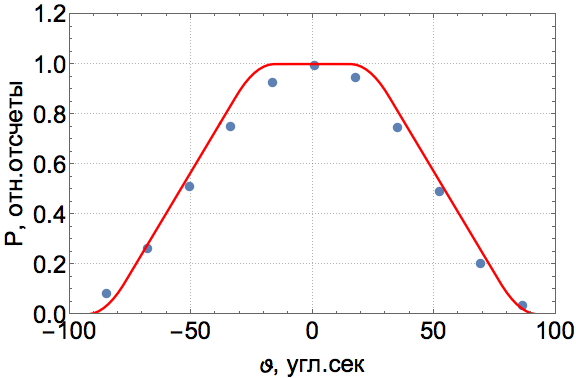
\includegraphics[width=0.3\textwidth]{images/zero_exp_300_300.png}} %$S_1 = 300$ мкм; $S_2 = 300$ мкм;
  \caption{Угловое распределение интенсивности в случае для системы из двух щелевых устройств, находящихся
  на расстоянии $L_1= 570 $мм и $L_2 = 1005$ мм; для первой и второй соответственно ($\delta = 0.1$ мм).
  (красная линия) - расчет, (синие точки) - эксперимент для (a) $S_1 = 20$ мкм; $S_2 = 40$ мкм,
  (b) $S_1 = 40$ мкм; $S_2 = 40$ мкм, (c) $S_1 = 50$ мкм; $S_2 = 100$ мкм,
  (d) $S_1 = 100$ мкм; $S_2 = 200$ мкм, (e) $S_1 = 100$ мкм; $S_2 = 300$ мкм,
   (f) $S_1 = 200$ мкм; $S_2 = 20$ мкм, (g) $S_1 = 200$ мкм; $S_2 = 200$ мкм,
   (h) $S_1 = 200$ мкм; $S_2 = 300$ мкм, (i) $S_1 = 300$ мкм; $S_2 = 300$ мкм }
  \label{ris:zero_exp}
\end{figure}

Исходя из полученных результатов наблюдается сходимость экспериментальных данных с расчетными.
Интеграл угловой функции сильно зависит от параметров схемы: расстояний между щелевыми коллиматорами и источником и
размеров щелевых коллиматоров. Анализа серии экспериментов позволил уточнить линейный размер источника $\delta = 0.1$мм,
значение которого было использовано во всех остальных расчетах.
